 
\documentclass{sig-alternate-2013}

\usepackage{url}
\usepackage[english,french]{babel}
\usepackage[utf8]{inputenc}
\usepackage{algorithm}
\usepackage{paralist}
\usepackage{algorithmicx}
\usepackage{algpseudocode}

\usepackage{fancyhdr}
\usepackage{graphicx}
\usepackage{hyperref}                                  
\usepackage{multirow}

\usepackage{epstopdf}
\usepackage{epsfig}

%% Bibtex
\usepackage[numbers]{natbib}

\usepackage{tikz}
\usetikzlibrary{plotmarks,shapes}

\usepackage{subcaption}

\newcommand{\TOFIX}[1]{\textcolor{orange}{#1}}
\newcommand{\TODO}[1]{\textcolor{red}{#1}}
\newcommand{\NAME}[0]{LSEQ}

%paralist
\renewcommand*\descriptionlabel[1]{%
\scshape #1}
\renewcommand\paradescriptionlabel[1]{%
\scshape #1}



\hypersetup{
  colorlinks,
  citecolor=black,
  filecolor=black,
  linkcolor=black,
  urlcolor=black
}

\title{\NAME{}: an Adaptive Structure for Sequences in Distributed
  Collaborative Editing}

\numberofauthors{1}
\author{
     \alignauthor Brice Nedelec, Pascal Molli, Achour Mostefaoui, Emmanuel Desmontils\\
     \affaddr{LINA, 2 rue de la Houssini\`ere}\\
     \affaddr{BP92208, 44322 Nantes Cedex 03}\\
     \email{first.last@univ-nantes.fr}
}

\newfont{\mycrnotice}{ptmr8t at 7pt}
\newfont{\myconfname}{ptmri8t at 7pt}
\let\crnotice\mycrnotice%
\let\confname\myconfname%

\permission{Copyright 2013 Association for Computing Machinery. ACM
  acknowledges that this contribution was authored or co-authored by an
  employee, contractor or affiliate of the national government of France. As
  such, the government of France retains a nonexclusive, royalty-free right to
  publish or reproduce this article, or to allow others to do so, for
  Government purposes only. Request permissions from permissions@acm.org.}
\conferenceinfo{DocEng'13,}{September 10--13, 2013, Florence, Italy.}
\copyrightetc{Copyright 2013 ACM \the\acmcopyr}
\crdata{978-1-4503-1789-4/13/09\ ...\$15.00.\\
  http://dx.doi.org/10.1145/2494266.2494278}


\clubpenalty=10000 
\widowpenalty = 10000

\date{}



%% DATA
%%\begin{filecontents}{avgWorstCase.data}
%%#nbInsert idsize 
%%100 4.16
%%200 7.65
%%300 11.32
%%500 18.7
%%800  29.35
%%1300  47.76
%%2100  76.63
%%\end{filecontents}
%%\begin{filecontents}{maxWorstCase.data}
%%# nbInsert  id size  
%%100 8
%%200 15
%%300 22
%%500 37
%%800 59
%%1300  90
%%2100  151
%%\end{filecontents}

\begin{filecontents}{avgWorstCase.data}
#nbInsert idsize  
5.0E-1 0.208 
1.0E0 0.3825
1.5E0 0.566
2.5E0 0.935
4.0E0 1.4675
6.5E0 2.379
1.05E1 3.83149
\end{filecontents}

\begin{filecontents}{maxWorstCase.data}
#nbInsert  idsize  
5.0E-1 0.4
1.0E0 0.75
1.5E0 1.1
2.5E0 1.85
4.0E0 2.95
6.5E0 4.5
1.05E1 7.55
\end{filecontents}

\begin{filecontents}{weissDataQueue.data}
#log nbInsert idsize  
2 0.2
3 0.584
3.69 2.5084
4 4.924

\end{filecontents}

\begin{filecontents}{weissDataFront.data}
#log nbInsert  idsize  
2 3.866
2.12 10
\end{filecontents}

\begin{filecontents}{weissDataRand.data}
#log nbInsert  idsize  
2 0.486
3 0.726
3.69 0.9
4 0.974
4.69 1.146
5 1.216
\end{filecontents}


\begin{filecontents}{roundrobinDataQueue.data}
#log nbInsert idsize  
2 0.2
3 0.966
3.69 4.714
4 9.508
\end{filecontents}

\begin{filecontents}{roundrobinDataFront.data}
#log nbInsert  idsize  
2 0.394
3 1.186
3.69 5.084
4 9.88
\end{filecontents}

\begin{filecontents}{roundrobinDataRand.data}
#log nbInsert  idsize  
2 0.442
3 0.682
3.69 0.85
4 0.924
4.69 1.092
5 1.164
\end{filecontents}


\begin{filecontents}{doubleDataQueue.data}
#log nbInsert idsize  
2 0.3982
3 0.9956
3.69 1.558
4 1.8328
4.69 2.5252
5 2.866
5.69 3.7334
\end{filecontents}

\begin{filecontents}{doubleDataFront.data}
#log nbInsert  idsize  
2 0.365
2.02 10
\end{filecontents}

\begin{filecontents}{doubleDataRand.data}
#log nbInsert  idsize  
2 0.2276
3 0.4088
3.69 0.542
4 0.608
4.69 0.768
5 0.84
5.69 1.018
\end{filecontents}


\begin{filecontents}{doubleroundrobinDataQueue.data}
#log nbInsert idsize  
2 0.5508
3 1.262
3.69 1.868
4 2.116
4.69 2.935
5 3.268
5.69 4.126
\end{filecontents}

\begin{filecontents}{doubleroundrobinDataFront.data}
#log nbInsert  idsize  
2 0.528
3 1.182
3.69 1.808
4 2.164
4.69 2.904
5 3.3
5.69 4.228
\end{filecontents}

\begin{filecontents}{doubleroundrobinDataRand.data}
#log nbInsert  idsize  
2 0.254
3 0.436
3.69 0.58
4 0.646
4.69 0.808
5 0.884
5.69 1.064
\end{filecontents}


\begin{filecontents}{doublerandomDataQueue.data}
#log nbInsert idsize  
2 0.5546
3 1.3186
3.69 2.27
4 2.566
4.69 3.298
5 3.65
5.69 4.15
6 4.436
\end{filecontents}

\begin{filecontents}{doublerandomDataFront.data}
#log nbInsert  idsize  
2 0.408
3 1.342
3.69 1.732
4 2.11
4.69 2.69
5 2.966
5.69 3.786
6 4.178
\end{filecontents}

\begin{filecontents}{doublerandomDataRand.data}
#log nbInsert  idsize  
2 0.248
3 0.426
3.69 0.56
4 0.6246
4.69 0.7894
5 0.864
5.69 1.044
6 1.1262
\end{filecontents}


%% DATA
%%\begin{filecontents}{1kInsertBase.data}
%%#nbInsert idsize 
%%2 71
%%3 66.1
%%4 67
%%5 59.4
%%6 59.14
%%7 49.4
%%8 47.5
%%9 37
%%10 35.2
%%11 27.58
%%12 24.9
%%13 26.9
%%14 28.9
%%15 30.9
%%16 32.9
%%17 34.9
%%18 37
%%19 38.9
%%20 40.9
%%30 60.9
%%40 80.99
%%\end{filecontents}

\begin{filecontents}{1kInsertBase.data}
1 7.1
1.5 6.61
2 6.7
2.5 5.94
3 5.91
3.5 4.94
4 4.75
4.5 3.7
5 3.52
5.5 2.758
6 2.49
6.5 2.69
7 2.89
7.5 3.09
8 3.29
8.5 3.49
9 3.7
9.5 3.89
10 4.09
15 6.09
\end{filecontents}

%%\begin{filecontents}{50kInsertBase.data}
%%#nbInsert idsize 
%%2 154.52
%%3 152.2
%%4 150.7
%%5 145.3
%%6 141.9
%%7 134.2
%%8 128.8
%%9 119.4
%%10 112.1
%%11 101
%%12 92.2
%%13 79.5
%%14 70.3
%%15 56.9
%%16 50.6
%%17 35
%%18 37
%%19 39
%%20 41
%%30 61
%%40 81
%%\end{filecontents}

\begin{filecontents}{50kInsertBase.data}
1 15.452
1.5 15.22
2 15.07
2.5 14.53
3 14.10
3.5 13.42
4 12.88
4.5 11.94
5 11.21
5.5 10.1
6 9.22
6.5 7.95
7 7.03
7.5 5.69
8 5.06
8.5 3.5
9 3.7
9.5 3.9
10 4.1
15 6.1
\end{filecontents}



%%% % %% % %%% %% % %% % %%% % %%% % %% % %% % % %%%
\begin{document}

%% Allocate sufficient space to include the full copyright in bottom left part
%% of the first page
%\makeatletter
%\renewcommand\@copyrightspace{
%\@float{copyrightbox}[b]
%\begin{center}
%\setlength{\unitlength}{1pc}
%\begin{picture}(20,9) %Space for copyright notice
%\put(0,-0.95){\crnotice{\@toappear}}
%\end{picture}
%\end{center}
%\end@float}
%\makeatother


\newtheorem{Def}{Definition}

\selectlanguage{english}

  \maketitle

  
\begin{abstract}
  Distributed collaborative editing systems allow users to work distributed in
  time, space and across organisations. Trending distributed collaborative
  editors such as Google Docs, Etherpad or Git have grown in popularity over
  the years. A new kind of distributed editors based on a family of distributed
  data structure replicated on several sites called Conflict-free Replicated
  Data Type (CRDT for short) appeared recently. This paper considers a CRDT
  that represents a distributed sequence of basic elements that can be lines,
  words or characters (sequence CRDT). The possible operations on this sequence
  are the insertion and the deletion of elements. Compared to the state of the
  art, this approach is more decentralised and scales better in terms of the
  number of participants. However, its space complexity is linear with respect
  to the total number of inserts and the insertion points in the document. This
  makes the overall performances of such editors dependent on the editing
  behaviour of users. This paper proposes and models \NAME{}, an adaptive
  allocation strategy for a sequence CRDT. \NAME{} achieves in the average a
  sub-linear spatial-complexity whatever is the editing behaviour. A series of
  experiments validates \NAME{} showing that it outperforms existing
  approaches.
\end{abstract}

  \category{I.7.1}{Document and Text
  Processing}{Document and Text Editing}[Document management]
\category{C.2.4}{Computer-Communication Networks}{Distributed
  Systems}[Distributed applications]
\category{D.2.8}{Software Engineering}{Metrics}[Complexity measures]


\keywords{Distributed Documents; Document Authoring Tools and Systems;
  Distributed Collaborative Editing; Real-time Editing; Conflict-free
  Replicated Data Types}

  \newpage
  \section{Introduction}

Distributed collaborative editing
systems~\cite{Ellis:1989:CCG:67544.66963,ellis1991groupware,greenberg1994real}
such as Google Docs, Etherpad or Git are now widely used and allow users to
work distributed in time, space, and across organizations. A new kind of
distributed editors~\cite{preguica2009commutative,weiss2007wooki} appeared
based on Conflict-Free Replicated Data Types
(CRDTs)~\cite{oster2006data,weiss2009logoot,shapiro2011conflict}. A CRDT is a
distributed data type replicated over several
sites~\cite{saito2005optimistic,saito2002replication}. A CRDT cannot implement
any centralized data structure but for instance can implement a counter, a set,
a tree, etc. In this paper we consider a special family or CRDTs that implement
a sequence of basic elements such as lines, words or characters that we call
\emph{sequence CRDT}. For our purpose and as a first step, we only consider two
basic operations on a sequence, the insert and the delete operations. Compared
to the state of the art, editors based on sequence CRDTs are more decentralized
and scale better. However, they have a linear space-complexity with respect to
the number of insertions. Consequently, they heavily depend on the editing
behaviour. Some editing scenarios lead to a permanent loss in performance.

In order to preserve the total order on the elements of the sequence, a unique
and immutable identifier is associated with each basic element of the structure
(character, line or paragraph according to the chosen granularity). This allows
to distinguish two classes of sequence CRDTs:
\begin{inparaenum}[(i)]
\item Fixed size identifier (also called the tombstones class). This class
  includes WOOT~\cite{oster2006data}, WOOTO~\cite{weiss2007wooki},
  WOOTH~\cite{ahmed2011evaluating}, CT~\cite{grishchenko2010deep},
  RGA~\cite{roh2011replicated},~\cite{Yu2012stringwise}. In this class, a
  tombstone replaces each suppressed element. Although it enjoys a fixed length
  for identifiers and it has a space complexity which depends on the number of
  operations. For example, a document with an history of a million operations
  and finally containing a single line can have as much as 499999
  tombstones. Garbaging tombstones requires costly protocols in decentralized
  distributed systems.
\item Variable-size identifiers. This class includes for example
  Logoot~\cite{weiss2009logoot}. It does not require tombstones, but its
  identifiers can grow unbounded. Consequently, although it does not require
  garbage protocols, its space complexity remains till now linear with the
  number of insert operations. Thus, it is possible to have only a single
  element in the sequence having an identifier of length
  499999. Treedoc~\cite{preguica2009commutative} uses both tombstones and
  variable size identifiers but relies on a complex garbage protocol when
  identifiers grow too much.
\end{inparaenum}

In this paper, we propose a new approach, called \NAME{}, that belongs to the
variable-size identifiers class of sequence CRDTs. Compared to the state of the
art, \NAME{} is an adaptive allocation strategy with a sub-linear upper-bound
in its spatial complexity. We experimented \NAME{} on synthetic sequences and
real documents. In both cases, \NAME{} outperforms existing approaches.

The remainder of the paper is organized as
follows. Section~\ref{sec:background} delineates the background on
variable-size identifiers class of sequence CRDTs and motivates this
work. Then, Section~\ref{sec:proposal} details \NAME{} and the three parameters
that control the growth and the selection of the identifiers. It describes each
parameter with its aim and its defect. Also, how their composition overcomes
their respective weaknesses. Section~\ref{sec:validation} validates the
approach by showing the effect of each one of the three parameters of \NAME{}
and also by comparing the proposed approach to Logoot. Finally,
Section~\ref{sec:relatedwork} reviews related works.

  \section{Preliminaries}
\label{sec:background}

Distributed collaborative editing systems consider a sequence of characters
replicated on $n$ sites. Each site manages a local copy of the sequence called
local replica. At some moments, the local replica can differ from some other
sites' local replica. Each site can $insert$ and $delete$ characters in the
sequence without any locking mechanism. Then, all sites exchange and deliver
the operations. When any site delivers an insert operation, the state of the
local replica may be different from the state of another replica.

The system is correct if:
\begin{inparaenum}[(i)]
\item It converges i.e. all local replicas of the sequence are equal when the
  system is idle. It corresponds to the eventual consistency
  property~\cite{johnson1975maintenance}.
\item It preserves all partial order relations $\prec$ between characters. If a
  site inserts the character $x$ between the characters $a$ and $b$ ($a \prec x
  \prec b$), this relation is preserved on each sites' replica. It
  corresponds to the property of intention preservation in Operational
  Transformation algorithms~\cite{sun1998achieving} used by Google Docs.
\end{inparaenum}

Let us illustrate this with an example. Assume that all the replicas of a
sequence of characters are equal and that the sequence looks like
$...abcd...$. Consider that a site inserts the character $e$ between $b$ and
$c$ and also consider that at the same moment, another site inserts a character
$f$ between $b$ and $c$. It results in two relations $b \prec e \prec c$ and $b
\prec f \prec c$. Once every site has delivered all the changes on their local
replica, the union of these two relations merges into a partial relation
without any precedence between $e$ and $f$. Consequently, two final states are
possible $abefcd$ and $abfecd$. The role of the sequence CRDTs is to build a
linear extension of the partial order formed by the intentions of all users to
obtain a unique total order.

Variable-size sequence CRDTs encode order relations into identifiers. For
example, the operation $insert(a=10 \prec x \prec b=15)$ can be sent as
$insert(x,12)$. This strategy does not require keeping tombstones, however it
is easy to see that identifiers can grow quickly and significantly degrade the
overall performance of the system. In the worst case, the system requires to
rebalance identifiers implying the use of a consensus algorithm.

In this paper, we focus on keeping the identifiers as small as possible hence
avoiding any costly protocol to rebalance them. Definition~\ref{def:model}
states a document as a set of pairs $(elt, id)$ where $elt$ can be a character
or a line and $id$ are unique immutable identifiers defined on the set of all
possible identifiers $\mathcal{I}$. $\mathcal{I}$ has an order relation $<$
which is dense and strictly totally ordered i.e. if $x,y \in \mathcal{I}$ and
$x < y$ then $\exists z \in \mathcal{I}, z\neq x, z\neq y, x < z <
y$. $alloc(p,q)$ is the allocation strategy function that generates $id \in
\mathcal{I}$. In Definition~\ref{def:id}, we state that an $id$ is a sequence
of numbers, $id_1<id_2$ if $id_1 $ precedes $id_2$ in lexicographic order. This
sequence is an efficient way to represent a dense order.

\begin{Def}[Model of a document]\ \\
A document is a set $\mathcal{D} = \{ (elt, id) \}$ with two operations:
\begin{itemize}
  \item insert($p \in \mathcal{I}$, elt, $q \in
    \mathcal{I}$):- $\mathcal{D} \cup \{(elt,id_{elt})\}$ \\ where
    $id_{elt}=alloc(p,q)$ with $p<id_{elt}<q$
  \item delete($id \in \mathcal{I}$):- $\mathcal{D}/\{(elt,id)\}$
\end{itemize}
\label{def:model}
\end{Def}

\begin{Def}[Variable-size identifier]
  A variable-size identifier $id$ is a sequence of numbers $id=[p_1.p_2\ldots
    p_n]$ which can designate a path in a tree~\footnote{Identifiers should
    include site ID to ensure the uniqueness property. However, for clarity
    purposes and in order to focus on allocation strategy, we did not
    include any site ID in this definition.}.
\label{def:id}
\end{Def}

In Figure~\ref{fig:treeexample}, we represent a document as a tree where each
identifier is a path from the root to a leaf. In this example, each level has a
maximum capacity (arity of the tree node) set to 100. A leaf is an element of
the sequence. For instance, $[10.13]$ is an identifier referencing the element
$b$.  Assume a user wants to insert an element $z$ between two existing
elements identified by $p$ and $q$:
\begin{asparaitem}
\item if $p=[11]$ and $q=[14]$, there is room for insertion. Both identifiers
  $[12]$ and $[13]$ are valid choices for the new element.
\item if $p=[14]$ and $q=[15]$, there is no room at this level. Since the model
  does not have further levels, the allocation function $alloc$ initiates a new
  level. Then, it chooses among this bunch of newly available identifiers:
  between $[14.0]$ and $[14.99]$.
\end{asparaitem}

\begin{figure}[h]
\begin{center}
\begin{tikzpicture}[scale=1.0]
\tiny

  
  \draw (0,0) -- node[anchor=south east]{0}  (-85pt, -50pt);
  \draw (0,0) -- node[anchor=south west]{99} ( 85pt, -50pt);

  \draw (0,0) -- node[anchor=east]{10} (-40pt, -50pt);
  \draw (0,0) -- node[anchor=east]{11} (  0pt, -50pt);
  \draw (0,0) -- node[anchor=east]{14} ( 30pt, -50pt);
  \draw (0,0) -- node[anchor=east]{15} ( 60pt, -50pt);

  \draw[fill=white] (0,0) circle (1pt);

\small
  \draw[fill=white] (-85pt, -50pt) node[anchor=north]{Begin} circle (1pt);
  \draw[fill=white] ( 85pt, -50pt) node[anchor=north]{End} circle (1pt);

\tiny
  \draw (-40pt,-50pt) -- node[anchor=east]{13} (-34.8pt, -100pt);
%  \draw (-40pt,-50pt) -- (-30.8pt, -100pt);
  \draw (-40pt,-50pt) -- node[anchor=west]{42} (-23.2pt, -100pt);
%  \draw (-40pt,-50pt) -- (-12.0pt, -100pt);
  \draw (-40pt,-50pt) -- node[anchor=west]{92}(- 3.2pt, -100pt);

\small
  \draw[fill=white] (-40pt, -50pt) node[anchor= east]{\TODO{a}} circle (1pt);
  \draw[fill=white] (  0pt, -50pt) node[anchor= north]{\TODO{e}} circle (1pt);
  \draw[fill=white] ( 30pt, -50pt) node[anchor= north]{\TODO{f}} circle (1pt);
  \draw[fill=white] ( 60pt, -50pt) node[anchor= north]{\TODO{g}} circle (1pt);

  \filldraw[black](-34.8pt, -100pt) node[anchor= north]{\TODO{b}} circle (1pt);
%  \filldraw[black] (-30.8pt, -100pt) node[anchor=north]{23} circle (1pt);
  \filldraw[black](-23.2pt, -100pt) node[anchor= north]{\TODO{c}} circle (1pt);
%  \filldraw[black] (-12.0pt, -100pt) node[anchor=north]{70} circle (1pt);
  \filldraw[black](- 3.2pt, -100pt) node[anchor= north]{\TODO{d}} circle (1pt);

\end{tikzpicture}

\caption{Underlying tree model of a variable-size identifiers sequence CRDT.
  Depth-1 contains four identifiers $[10]$, $[11]$, $[14]$ and $[15]$ labeling
  the elements $a$, $e$, $f$ and $g$ respectively. Also, depth-1 contains the
  bounds of the sequence $\langle [0], Begin \rangle$ and $\langle [99],End
  \rangle$. Depth-2 contains three identifiers $[10.13]$, $[10.42]$, and
  $[10.92]$ labeling $b$, $c$ and $d$ respectively.  }
\label{fig:treeexample}
\end{center}
\end{figure}


\begin{figure*}
\centering
\begin{subfigure}[t]{0.47\textwidth}
  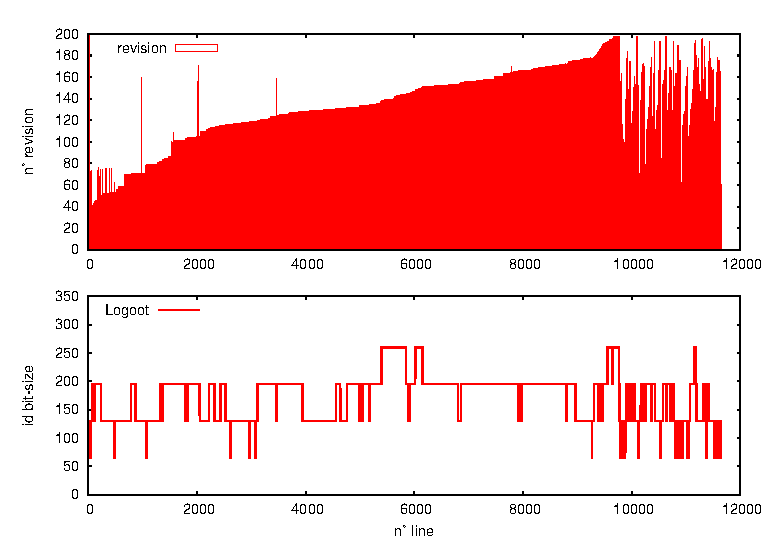
\includegraphics[width=\textwidth]{img/compliant.eps}
  \caption{A page of 12k lines mostly edited at
    the end.}
  \label{im:posteonlyblue}
\end{subfigure}
\begin{subfigure}[t]{0.47\textwidth}
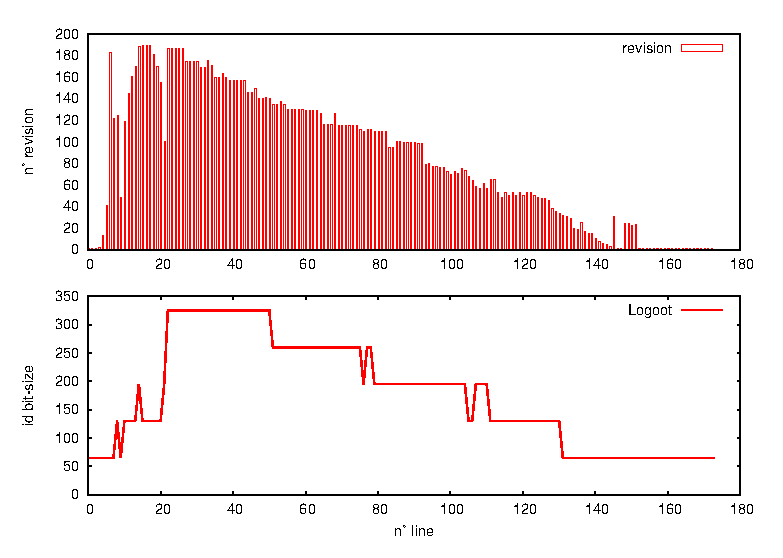
\includegraphics[width=\textwidth]{img/motivating.eps}
\caption{A page of 170 lines mostly edited at the beginning.}
\label{im:didyouknowonlyblue}
\end{subfigure}
\caption{Experiments made on a Wikipedia pages. The top figure shows the
  spectrum of the page (revision number of each line). The bottom figure shows
  the bit-lenght of the identifier assigned to each line. The allocation
  strategy is $boundary$ from the Logoot approach.}
\end{figure*}

\subsection{Allocation strategies}
The Logoot paper~\cite{weiss2009logoot} already highlighted the importance of
allocation strategies ($alloc$). Indeed, experiments concerned two strategies.
\begin{inparaenum}[(1)]
\item \emph{Random}: randomly choosing between the identifiers of the two
  neighbours. It delivers poor performance because the identifiers quickly
  saturate the space, resulting in the creation of new levels. As consequence,
  the size of identifiers grows quickly.
\item \emph{Boundary}: randomly choosing between the identifiers of the two
  neighbours bounded by a $boundary$ maximum value. The strategy allocates the
  new identifiers closer to their preceding identifier. Of course, it works
  well when the editions are performed right-to-left.
\end{inparaenum}

Figures~\ref{im:posteonlyblue} and~\ref{im:didyouknowonlyblue} show the editing
behaviour of two Wikipedia pages. The top part shows the spectrum associated
with the pages. A spectrum gives an overview of the editing behaviour
associated with a page. The spectrum gives the revision number of each line of
a document, i.e., the relative date of their insert operation.  As the left
spectrum suggests, most of the insert operations situates the new elements at
the end of the document, i.e., the last lines of the page are more recent. On
the opposite, the second spectrum shows that most of the insert operations
situates the newest elements at the beginning of the document.  The bottom
figures associate the bit-length of the identifier of each line of the document
using the \emph{boundary} strategy. In the first figure, we consider a page of
$12k$ lines. Identifiers do not exceed $256$ bits and they are well spread
between levels $[1-4]$. It leads to a satisfying average of $169.7$ bits/id. On
the contrary, the editing behaviour on the second document (see
figure~\ref{im:didyouknowonlyblue}) that has only 170 lines does not fulfills
the right-to-left editing behaviour assumed by the \emph{boundary} strategy. In
this case, we observe, on an existing document, the worst-case of linear growth
of the size of identifiers.  The average bit-length is $172.25$ bits/id over 5
levels.

\subsection{Issues and motivations}
Most of existing CRDTs' allocation strategies make the assumption of
right-to-left and top-to-bottom editing behaviour. This strong hypothesis
allows better space management but other behaviours may lead to a quick
decrease in performance. Therefore, it makes the distributed collaborative
editor unsafe.

In order to build an efficient distributed collaborative editor based on a
sequence CRDT, we need an adaptive allocation function $alloc$, i.e., an
allocation strategy independent of an editing behaviour. \emph{The
  unpredictability of the editing behaviour makes the allocation of identifiers
  challenging. At any time, the CRDT knows what happened in the past and the
  current operations. Still, inferring the upcoming operations is complex if
  not impossible.}

\begin{Def}[Problem statement]\ \\
Let $\mathcal{D}$ be a document on which $n$ insert operations have been
performed.  Let $\mathcal{I}(\mathcal{D})= \{id |
(\_,id)\in{\mathcal{D}}\}$. The function $alloc(id_p,id_q)$ should provide
identifiers such as:
\begin{center}
$\sum\limits_{id \in \mathcal{I}} { {log_2(id)}\over{n}}$ $< O(n)$
\end{center}
\end{Def}

The problem statement concerns the allocation function $alloc$ which should
have a sub-linear upper-bound in its space complexity. Such function would
greatly improve the current state of art since the document does not require
any additional costly protocol: the average size of identifiers being under an
acceptable bound.

  \section{\NAME{} Allocation Function}
\label{sec:proposal}

\NAME{} applies a very simple strategy: each time we create a new depth in the
tree between two identifiers $p$ and $q$, we double the base of this depth and
we choose randomly a strategy among \emph{boundary+} or
\emph{boundary--}. \emph{boundary+} allocates from $p$ plus a fixed boundary,
\emph{boundary--} allocates from $q$ minus a fixed boundary. The boundary never
changes whatever the depth of the tree.

The following idea is the foundation of this approach: as it is complex to
predict the editing behaviour, the principle is to sacrifice some depths of the
tree with the insurance that the reward will compensate the loss.  In other
words, if \NAME{} chooses the wrong strategy at a given depth, it will
eventually choose the right one in the next depths. Since it doubles the base
at each new depth, when the right strategy will be found, it will overwhelm the
cost of lost depths.

\subsection{Base Doubling}
Logoot's~\cite{weiss2009logoot} underlying allocation strategy always uses the
same base to allocate its identifiers. With regard to the tree representation,
it means that the arity is set to $base$. A high base value is not profitable
if the number of insert operations in this part of the sequence is low. On the
contrary, keeping a constant base value when the number of insert operations
starts to be very high does not allow to fully benefit of the \emph{boundary}
strategy. For instance, in Figure~\ref{im:posteonlyblue} the Wikipedia page has
12k lines that justifies the usage of a large base unlike
Figure~\ref{im:didyouknowonlyblue} with only 170 lines. Knowing the dilemma,
the objective is to adapt the base according to the number of insertions in
order to make a better reflection of the actual size of the document.  Since it
is impossible to \emph{a priori} know the size of the document, the idea is to
start with a small base due to the empty sequence, and then to double it when
and where necessary, i.e. when the depth of identifiers increases.

%\input{input/basealgo.tex}

Doubling the base at each depth implies an exponential growth of the number of
available identifiers. Thus, the model corresponds to the exponential
trees~\cite{andersson2007dynamic,singh2011implementation,andersson1996faster}
and consequently it benefits of their complexities. An exponential tree of
depth $k$ can store up to $N_k=N_{k-1}+k*k!$ identifiers where $N_1=base$.  In
other words, the arity of a node depends of its depth: a node has twice more
children than its parent node, and the root has $base$ children.

%%Algorithm~\ref{algo:doubledbase} computes the base at a given depth.
Knowing this exponential tree model, the binary representation of the
identifier is $\Sigma_{i=1}^{id.size} b*2^i$ where $b$ is the initial base
(conveniently a power of 2). Practically, if the initial base is $2^4$ then,
there are $2^{4+1}$ possibilities to choose an identifier at depth 1, $2^{4+2}$
at depth 2, etc.

The base doubling relies on the following assumption: it is the lack of space
that triggers the growth of identifiers. Therefore, an inefficient allocation
strategy will entail an excessive growth of the identifier size as the system
doubles the base anyway and the lost depths are more and more costly.

\subsection{Allocation Strategies}

\cite{weiss2009logoot} introduced two allocation strategies: \emph{boundary}
and \emph{random}. In the experiments, the former outperforms the
latter. Despite this, the \emph{boundary} strategy is heavily application
dependent. If a user mainly performs insert operations in the end of the
document the allocation will perform well. However, front editing will cause a
quick linear growth of the size of identifiers.

In \NAME{}, we introduce the allocation strategy named
\emph{boundary--}. Basically, this strategy is the opposite of the original
\emph{boundary} strategy. In this paper, we rename \emph{boundary} to
\emph{boundary+}. Let us consider an insert operation between two elements with
the identifiers $p$ and $q$. While the \emph{boundary+} strategy preferably
allocates a position near the preceding identifier $p$, the \emph{boundary--}
strategy allocates a position near the succeeding identifier $q$. Indeed,
\emph{boundary--} starts from position $q$ and subtracts a boundary value
instead of starting from position $p$ and add a boundary value. The arithmetic
operation explains the names given to theses
strategies. Figure~\ref{img:positionchoice} shows the results obtained by these
two strategies with the same neighbours and random value. The left figure shows
the \emph{boundary+} strategy which ends up with $[50.11]$ while the right
figure shows the \emph{boundary--} strategy which ends up with $[50.89]$. They
leave free space for future insertions of 88 identifiers in the end and in
front respectively.

\begin{figure}[h]
\begin{center}
%%\fbox{
\begin{tikzpicture}[scale=0.745,cap=round]
\small

%% Titles
  \draw (5.5,82pt) -- node[anchor=east]{boundary+} (5.5,82pt);
  \draw (5.5,82pt) -- node[anchor=west]{boundary-} (5.5,82pt);

\tiny
%% Boundary +
  \draw [<-] (2.625,-16pt)--( 2.625, -26pt)  node[anchor=north] {insertion};

  \draw  (1.25,60pt)-- ( 3.75, 60pt);
  \draw  (0,0)-- (5, 0);
  
  \draw [dashed] (2.5,3pt) to[out=90,in=280] (1.25,55pt);
  \draw [->,ultra thick,dashed] (2.5,3pt) to[out=90,in=280] (1.6,55pt);
  \draw [dashed] (2.85,3pt) to[out=90,in=280] (3.75,55pt);  
  
  \draw [->,thick,color=red] (1.25,77pt) -- node[anchor=south]{$+20$}
  (1.9,77pt);
  \draw [dashed, color=red] (1.9,77pt) -- (1.9,57pt);


  \draw (0,1pt) -- (0,-3pt) node[anchor=north] {0};
  \draw (5,1pt) -- (5,-3pt) node[anchor=north] {$100$};
  \draw (1.25,57pt) -- (1.25,61pt) node[anchor=east] {0};
  \draw (1.6,57pt) -- (1.6,61pt) node[anchor=south] {\textbf{11}};
  \draw (3.75,57pt) -- (3.75,61pt) node[anchor=west] {$100$};
  \draw (2.5,1pt) -- (2.5,-3pt) node[anchor=north] {\textbf{50}};
  \draw (2.85,1pt) -- (2.85,-3pt) node[anchor=north] {$51$};


%% Delimitation
  \draw [thick] (5.5,-40pt) -- (5.5, 90pt);

%% Boundary -
  \draw [<-] (8.625,-16pt)--( 8.625, -26pt)  node[anchor=north] {insertion};

  \draw  (7.25,60pt)-- ( 9.75, 60pt);
  \draw  (6,0)-- (11, 0);
  
  \draw [dashed] (8.5,3pt) to[out=90,in=280] (7.25,55pt);
  \draw [->,ultra thick,dashed] (8.5,3pt) to[out=90,in=280] (9.4,55pt);
  \draw [dashed] (8.85,3pt) to[out=90,in=280] (9.75,55pt);  

  \draw [->,thick,color=red] (9.75,77pt) -- node[anchor=south]{$-20$}
  (9.1,77pt);
  \draw [dashed, color=red] (9.1,77pt) -- (9.1,57pt);
  
  \draw (6,1pt) -- (6,-3pt) node[anchor=north] {0};
  \draw (11,1pt) -- (11,-3pt) node[anchor=north] {$100$};
  \draw (7.25,57pt) -- (7.25,61pt) node[anchor=east] {0};
  \draw (9.4,57pt) -- (9.4,61pt) node[anchor=south] {\textbf{89}};
  \draw (9.75,57pt) -- (9.75,61pt) node[anchor=west] {$100$};
  \draw (8.5,1pt) -- (8.5,-3pt) node[anchor=north] {\textbf{50}};
  \draw (8.85,1pt) -- (8.85,-3pt) node[anchor=north] {$51$};


\end{tikzpicture}
%%}

\caption{Choice of the digit part of identifiers in \emph{boundary+} (left) and
  \emph{boundary-} (right). In both case: constant base set to $100$,
  boundary value set to $20$ and the random number is $11$. The results are
  $[50.11]$ (\emph{boundary+}) and $[50.89]$ (\emph{boundary-}).}
\label{img:positionchoice}
\end{center}
\end{figure}


As expected, while the \emph{boundary+} algorithm handles the end editing,
the \emph{boundary--} algorithm aims the front editing. They both have
an antagonist weakness. Thus, \emph{boundary--} cannot be used alone safely,
just like \emph{boundary+}.

\subsection{Strategy choice}

Current variable-size sequence CRDTs rely on a unique strategy that is not
versatile in the sense that it does not adapt to every editing behaviour. As it
is impossible to \emph{a priori} know the editing behaviour and then, obtain
the perfect solution to any sequences, \NAME{} randomly alternates between
\emph{boundary+} and \emph{boundary--}. Thus, when \NAME{} increases the
identifier size, it has $1\over{2}$ chance to choose either \emph{boundary+} or
\emph{boundary--}. This kind of choice implies lost depths but the main idea
is: some depths are lost indeed, nevertheless it is acceptable if the reward
compensate the losses.

%%%%%%% CHOOSE THE POSITION IN DENSE SPACE MANG %%%%%%%%
\begin{algorithm}[h]
\small
\algrenewcommand{\algorithmiccomment}[1]{\hskip2em$\rhd$ #1}

  \begin{algorithmic}[1]
  \State \textbf{let} $boundary := 10;$ \Comment{Any constant} 
  \State \textbf{let} $\mathcal{S} := \{\}$; 
  \Comment{map<depth,boolean>}
  \State \Comment{$true$: $boundary+$} 
  \State \Comment{$false$: $boundary-$} 
  \State

    \Function{alloc}{p, q $\in \mathcal{I}$}
    
      \State \textbf{let} $depth := 0$; $interval := 0$;

      \While{$(interval < 1)$} \Comment{Not enough for 1 insert}
        \State $depth++$;
        \State $interval := prefix(q,depth) - prefix(p,depth) -1$;
      \EndWhile
      
      \State \textbf{let} $ste p:= min(boundary,interval)$; \Comment{Process 
        the maximum step to stay between $p$ and $q$}

      \If{$not(\mathcal{S}.exist(depth))$} \Comment{add the new entry}
        \State \textbf{let} $rand := RandBool()$;
        \State  $\mathcal{S}.set(depth, rand)$;
      \EndIf
      \If{$\mathcal{S}.get(depth)$} \Comment{$boundary+$}
        \State \textbf{let} $addVal := RandInt(0,step)+1$;
        \State \textbf{let} $id := prefix(p,depth) + addVal$;
      \Else \Comment{$boundary-$}
        \State \textbf{let} $subVal := RandInt(0,step)+1$;
        \State \textbf{let} $id := prefix(q,depth) - subVal$;
      \EndIf

      \State \textbf{return} $id$;
    \EndFunction
    
    \State

    \Function{prefix}{id $\in \mathcal{I}$, depth $\in \mathbb{N}^*$}
      \State \textbf{let} $idCopy := [\ ]$;
      \For{($cpt:=1$ to $depth$)}
        \If{($cpt<id.size$)} \Comment{Copy the value}
          \State $idCopy = idCopy.append(id.at(cpt))$;
          \Else \Comment{Add 0 encoded in the right base}
          \State $idCopy = idCopy.append(0_{base(cpt)})$; \label{line:base}
        \EndIf
      \EndFor
      \State \Return $idCopy$;
    \EndFunction

  \end{algorithmic}
\caption{\NAME{} allocation function}
\label{algo:strategychoicerandom}

\end{algorithm}


Algorithm~\ref{algo:strategychoicerandom} details the allocation function
\NAME{}. The depth-0 base value is $2^4$ and the \emph{boundary} to $10$. The
collection $\mathcal{S}$ which stores the strategy choices starts empty. Three
parts compose the algorithm.
\begin{inparaenum}[(1)]
  \item The first part processes the interval between the two identifiers $p$
    and $q$ at each depth until it is sufficient for at least one
    identifier. The step limits the interval where $alloc$ will allocate the
    new identifier.
  \item The second part determines the allocation strategy. If the function did
    not allocate any identifiers at this depth yet, it randomly chooses among
    \emph{boundary+} and \emph{boundary--}. Then it saves this choice for
    future decisions in $\mathcal{S}$.
  \item The final part of the algorithm constructs the new
    identifier. Depending on the strategy, it randomizes a value using the
    $step$ previously processed, and adds/subtracts this random value to the
    $prefix$ of $p$/$q$ at the wanted depth. The $prefix$ function takes an
    identifier $id$ in argument, and copies it until it reaches $depth$. If the
    identifier size is smaller than the requested depth, the function appends a
    zero to the copy for each missing depth. Each number in the sequence that
    composes the identifier must be carefully encoded in the base depending on
    the depth. Line~\ref{line:base} refers to $base(cpt)$. It is a very simple
    function that computes the base value at a given depth ($cpt$). Thus,
    $0_{base(cpt)}$ means that the binary representation of $0$ uses
    $log_2(base(cpt))$ bits. Consequently, the add and subtract operations do
    not require more efforts than regular arithmetic operations.
\end{inparaenum}

Figure~\ref{fig:lseqtreeexample} illustrates the allocation strategy \NAME{} by
showing its underlying tree model. First the empty sequence contains only two
identifiers: the beginning ($[0]$) and the end ($[31]$). The sequence needs
three additional identifiers between $[0]$ and $[31]$. First, \NAME{} randomly
assigns an allocation strategy to the depth $1$: \emph{boundary+}. Then, it
employs this strategy to allocate the three new identifiers ($[9]$, $[10]$,
$[23]$). The randomness makes the first and second element very close in term
of identifier distance.  Unfortunately, the sequence requests three other
identifiers between these two. Consequently, the depth has to grow to contain
these new elements. Since \NAME{} did not use any strategy at this depth yet,
it must randomly choose one. Here, the choice is \emph{boundary--}. Therefore,
this strategy allocates the three new identifiers. Furthermore, the underlying
exponential tree model extends the number of possible identifiers to $64$. In
this example, the resulting fresh identifiers are $[9.32]$, $[9.51]$ and
$[9.60]$.


\begin{tikzpicture}[scale=0.95]
\tiny

  \draw (-100pt,0)node[anchor=north east]{\textbf{Strategy}\ \ \ \ }--
        (-100pt,-120pt);
  \draw (-145pt,0)node[anchor=north east]{\textbf{Base}\ }--
        (-145pt,-120pt);
  \draw (-100pt, -25pt) node[anchor=east]{$boundary+$} -- (-100pt, -25pt);
  \draw (-145pt, -25pt) node[anchor=east]{$32$} -- (-145pt, -25pt);
  \draw (-100pt, -75pt) node[anchor=east]{$boundary-$} -- (-100pt, -75pt);
  \draw (-145pt, -75pt) node[anchor=east]{$64$} -- (-145pt, -75pt);
  \draw (-100pt,-110pt) node[anchor=east]{$???$} -- (-100pt,-110pt);
  \draw (-145pt,-110pt) node[anchor=east]{$128$} -- (-145pt,-110pt);
  \draw[dashed] (-170pt,- 50pt) -- (70pt,- 50pt);
  \draw[dashed] (-170pt,-100pt) -- (70pt,-100pt);


  \draw (0,0) -- node[anchor=east]{0}   (-70pt, -50pt);
  \draw (0,0) -- node[anchor=west]{31}  ( 70pt, -50pt);

  \draw (0,0) -- node[anchor=east]{9}  (-50pt, -50pt);
  \draw (0,0) -- node[anchor=west]{10} (  0pt, -50pt);
  \draw (0,0) -- node[anchor=west]{23} ( 30pt, -50pt);

  \draw (-50pt, -50pt) -- (-25.0pt, -100pt);
  \draw (-50pt, -50pt) -- (-10.2pt, -100pt);
  \draw (-50pt, -50pt) -- (- 3.2pt, -100pt);

  \draw[fill=white] (0,0) circle (1pt);

  \draw[fill=white] (-70pt, -50pt) node[anchor=south east]{Begin} circle (1pt);
  \draw[fill=white] ( 70pt, -50pt) node[anchor=south west]{End} circle (1pt);

  \draw[fill=white] (-50pt, -50pt) circle (1pt);
  \draw[fill=white] (  0pt, -50pt) circle (1pt);
  \draw[fill=white] ( 30pt, -50pt) circle (1pt);

  
  \filldraw[black] (-25.0pt, -100pt) node[anchor=south east]{32} circle (1pt);
  \filldraw[black] (-10.2pt, -100pt) node[anchor=south east]{51} circle (1pt);
  \filldraw[black] (- 3.2pt, -100pt) node[anchor=south west]{60} circle (1pt);

\end{tikzpicture}



This example highlights the major principle of \NAME{}.
Figure~\ref{fig:lseqtreeexample} depicts an exponential tree model that clearly
grows in arity over depths. It means more and more available identifiers when
the tree grows. This design aims to adjust the depth of the tree to the number
of insert operations. The next section aims to demonstrate experimentally that
\NAME{} achieves sub-linear space complexity in extreme setups and also
outperforms best CRDTs on real documents.


  \section{Experimentation}
\label{sec:validation}

This experimentation section is comprised of two parts. The first part focuses
on highlighting the behaviour of \NAME{} on extreme cases. The measurements
capture the effect of a large number of insert operations on the identifier
sizes. We synthesized different editing behaviours. Analyses are made step by
step to bring out the contribution of each component to \NAME{}. Previous
experiments~\cite{ahmed2011evaluating,preguica2009commutative,weiss2009logoot}
focused on average setups and did not consider such extreme setups.

The second part of experiments aims to validate if \NAME{} also performs well
on average setups.  In order to do so, we compare Logoot identifiers to \NAME{}
identifiers on representative Wikipedia pages with antagonist editing
behaviours. We choose Logoot as it delivers overall best performances for
variable-size sequence CRDTs according to~\cite{ahmed2011evaluating}.

The experiments focus on the digit part of identifiers. Indeed, the source and
clock part of identifiers are common to all the variable-size identifiers
approaches. They do not impact on the complexity and can be drastically
compressed. Consequently, it is the digit part that reflects the significant
improvements.

To evaluate \NAME{} performance, we developed a Java framework called LSEQ and
released the source on GitHub platform under the terms of the GPL
licence~\footnote{\url{https://github.com/Chat-Wane/LSEQ}}.

\subsection{Synthetic Documents Experiments}
\label{ssec:components}

We designed three experimental setups of synthetic sequences, namely monotone
editing behaviour in one position (first and last position), and totally random
insertions. The monotonic insertions algorithms choose a particular element and
continuously insert new elements before/after this element. For the front
editing, it targets the beginning of the document and inserts
continuously after it. The end editing, it targets the end of the
document and inserts continuously before it. The random behaviour randomly
inserts elements in the range $[0-doc.size[$. The insertions algorithms perform
a large number of insert operations on the sequence (up to
$10^6$). Furthermore, each operation only concerns one element at a time.

In these experiments, we measure the average bit-length of the digit part of
identifiers on four different configurations. In order of appearance: a simple
\emph{boundary+} strategy (\textbf{B}), a base doubling (\textbf{D}) at each
new depth, a Round-Robin strategy choice (\textbf{RR}) and a random strategy
choice with base doubling (\textbf{\NAME}).

\paragraph{Boundary \textbf{B} Experiment}

\begin{figure}
\begin{center}
\small
\begin{tikzpicture}[scale=0.7,x=1.57cm, y=0.6cm,font=\sffamily]
%Axis
    \draw[->] (0,0) -- coordinate (x axis mid) (6.5,0);
    \draw[->] (0,0) -- coordinate (y axis mid) (0,10.5);
%Ticks
    	\foreach \x        in { 0,
                              1,
                              2,
                              3,
                              4,
                              5,
                              6}
                              {
     		\draw (\x,1pt) -- (\x,-3pt) node[anchor=north] {\x};}

     	\foreach \y/\ytext in { 0/0,
                              1/,
                              2/,
                              3/150,
                              4/,
                              5/,
                              6/300,
                              7/,
                              8/,
                              9/450,
                              10/} {
     		\draw (1pt,\y) -- (-3pt,\y) node[anchor=east] {\ytext} ;}
%Labels      
	\node[below=0.3cm] at (x axis mid) {$log_{10}(nbInsert)$};
        \node[rotate=90, below=-1.0cm] at (y axis mid) {\textbf{id
            bit-length}};

%Plots
	\draw plot[mark=*, mark options={fill=black}] file
              {weissDataQueue.data}; \draw plot[mark=triangle*, mark
                options={fill=black} ] file {weissDataFront.data}; \draw
              plot[mark=square*, mark options={fill=black}] file
              {weissDataRand.data};

    
	%legend
	\begin{scope}[shift={(4,8)}] 
	\draw (0,0) -- plot[mark=*, mark options={fill=black}] (0.25,0) --
        (0.5,0) node[right]{End editing}; \draw[yshift=\baselineskip] (0,0)
        -- plot[mark=triangle*, mark options={fill=black}] (0.25,0) -- (0.5,0)
        node[right]{Front editing}; \draw[yshift=2*\baselineskip] (0,0) --
        plot[mark=square*, mark options={fill=black}] (0.25,0) -- (0.5,0)
        node[right]{Random editing};
	\end{scope}

\end{tikzpicture}

\caption{Simple \emph{boundary+} setup (\textbf{B}) with $base=2^{10}$ and
  $boundary=10$}
\label{fig:dimlogexperiment}
\end{center}
\end{figure}

\begin{asparadesc}
\item[Objective:] to show that \emph{boundary+} does not adapt itself neither
  to any monotonic editing behaviour nor to the number of insert
  operations. The expected space complexity is linear compared to the number of
  inserts in any monotonic editing behaviour. The random editing should lead to
  a logarithmic size of identifiers.

\item[Description:] the measurements concern the average bit-length of the
  digit part of identifiers. The checkpoints are 100, 1000, 5000, 10000, 50000,
  100000 insert operations. The experimental setup is \textbf{B} with the
  following parameter values: a \emph{boundary+} strategy with $boundary=10$
  and a constant $base=2^{10}$. It corresponds to the Logoot approach with
  lower values.

\item[Results:] Figure~\ref{fig:dimlogexperiment} shows on the x-axis
  the number of insertions with a logarithmic scale and on y-axis the
  average bit-length of identifiers. As expected the identifiers size
  grows when the number of insertions increases. \textbf{B} handles
  the random editing behaviour with a logarithmic average growth of
  its identifiers. However, with both front and end editing
  behaviour, the curve is linear compared to the number of insertions.
  The end editing remains acceptable in comparison of front editing,
  but the linear growth would eventually lead to the need of a costly
  re-balance protocol.

\item[Reasons:] The front and end editing behaviours tend to unbalance the
  underlying tree model of \textbf{B}. The \emph{boundary+} allocation strategy
  has been designed to handle edition at the end. It reserves more space
  for identifiers at the end, predicting future insertions. The obverse is less
  space for identifiers at front, therefore the front editing behaviour
  unbalances the tree even more quickly (leading to a worst-case space
  complexity of the total identifier size of $O(nb\_insert^2)$). For the same
  reason, the random editing behaviour leads to logarithmic space complexity:
  the tree model is balanced.
\end{asparadesc}

\paragraph{Base doubling \textbf{D} experiment}

\begin{asparadesc}
\item[Objective:] to show that \textbf{D} is not suitable in any case because
  it does not adapt on the editing behaviour.  However, it constitutes an
  improvement over \textbf{B} due to its scalability in terms of insertions
  number.  Indeed, it has a sub-linear upper-bound when the editing behaviour
  is the expected one. Since \textbf{D} uses a \emph{boundary+} allocation
  strategy, the sub-linear upper-bound is on the end editing. On the other
  hand, the expectation on the front editing is even worse than the first
  experiment (with \textbf{B}). The random editing should stay with its
  logarithmic shape unchanged.

\item[Description:] like the previous experiment, this experimentation concerns
  the average bit-length of identifiers. The \textbf{D} setup provides the new
  identifiers.  \emph{boundary+} and base doubling compose this setup. The
  variables are $boundary=10$ and a base starting from $base=2^{4+depth}$. The
  measures are taken at 100, 1000, 5000, 10000, 50000, 100000, 500000
  insertions.

\item[Results:] Figure~\ref{fig:doubleexperiment} shows on the x-axis the
  number of insertions on a logarithmic scale, and on the y-axis the average id
  bit-length. Like \textbf{B}, \textbf{D} provides constantly growing
  identifiers. When the editing behaviour is the expected one, the growth is
  sub-linear compared to the number of insertions. Otherwise, the growth is
  quadratic. Given this, \textbf{D} alone is better than \textbf{B} when the
  current editing behaviour is known. In our context where we have no prior
  knowledge of the editing behaviour, \textbf{D} alone is unsafe.

\item[Reasons:] the base doubling assumes that a high number of insertions
  triggered the creation of previous levels in the tree. Thus, it enlarges the
  number of available identifiers in the new level. If the insertions saturated
  the previous levels, then it verifies this hypothesis, resulting in an
  efficient allocation. Of course, if the base doubling hypothesis is false, in
  the worst case, each new level will contain only one identifier. Each one of
  these identifiers will have a space complexity equal to
  $\sum\limits_{i=1}^{n}{(log_2(b) + i)}$ where $n$ is the number of insertions
  and $b$ is the departure base.
\end{asparadesc}

\begin{figure}
\small
\begin{center}
\begin{tikzpicture}[scale=0.65,x=1.57cm,y=0.6cm,font=\sffamily]

%Axis
    \draw[->] (0,0) -- coordinate (x axis mid) (6.5,0);
    \draw[->] (0,0) -- coordinate (y axis mid) (0,10.5);
%Ticks
    	\foreach \x        in { 0,
                              1,
                              2,
                              3,
                              4,
                              5,
                              6}
                              {
     		\draw (\x,1pt) -- (\x,-3pt) node[anchor=north] {\x};}

     	\foreach \y/\ytext in { 0/0,
                              1/,
                              2/,
                              3/150,
                              4/,
                              5/,
                              6/300,
                              7/,
                              8/,
                              9/450,
                              10/} {
     		\draw (1pt,\y) -- (-3pt,\y) node[anchor=east] {\ytext} ;}
%Labels      
	\node[below=0.3cm] at (x axis mid) {$log_{10}(nbInsert)$};
        \node[rotate=90, below=-1.0cm] at (y axis mid) {\textbf{id
            bit-length}};
        
%Plot
  \draw plot[mark=*, mark options={fill=black}]
  file {doubleDataQueue.data};
  \draw plot[mark=triangle*, mark options={fill=black} ] 
  file {doubleDataFront.data};
  \draw plot[mark=square*, mark options={fill=black}] 
  file {doubleDataRand.data};
    
%legend
  \begin{scope}[shift={(4.5,8)}] 
    \draw (0,0) -- 
    plot[mark=*, mark options={fill=black}] (0.25,0) -- (0.5,0) 
    node[right]{End editing};
    \draw[yshift=\baselineskip] (0,0) -- 
    plot[mark=triangle*, mark options={fill=black}] (0.25,0) -- (0.5,0)
    node[right]{Front editing};
    \draw[yshift=2*\baselineskip] (0,0) -- 
    plot[mark=square*, mark options={fill=black}]  (0.25,0) -- (0.5,0)
    node[right]{Random editing};
  \end{scope}
\end{tikzpicture}

\caption{Base doubling setup (\textbf{D}) ($base=2^{4+id.size}$,
  $boundary=10$)}
\label{fig:doubleexperiment}
\end{center}
\end{figure}

\paragraph{Round-Robin alternation \textbf{RR} experiment}

\begin{asparadesc}
\item[Objective:] to show that a Round-Robin alternation between
  \emph{boundary+} and \emph{boundary--} provides identifiers with a linear
  upper-bound and consequently does not scale as regards the number of
  insertions.  However, it is an improvement over \textbf{B} and \textbf{D}:
  with no \emph{a priori} knowledge \textbf{RR} avoids the trivial worst case.

\item[Description:] the experiment focuses on the average bit-length of the
  digit part of identifiers. The configuration is a \textbf{RR} setup with two
  allocation strategies \emph{boundary+} and \emph{boundary--}. The parameters
  value are $boundary=10$, and a constant $base=2^{10}$. The measures are taken
  at 100, 1000, 5000, 10000, 50000, 100000 insertions.

\item[Results:] Figure~\ref{fig:roundrobinexperiment} shows on the x-axis on a
  logarithmic scale the number of insertions performed on the sequence. The
  y-axis presents the average bit-length of the digit part of identifiers.
  While on the random editing behaviour, the identifiers size curve stays in a
  logarithmic shape, front and end editing are both in linear shape. These
  observations mean that like \textbf{B}, \textbf{RR} does not adapt to the
  number of insertions, and, on the opposite of \textbf{B} and \textbf{D} it
  avoids the trivial worst case of front edition. Since every collaborative
  editing behaviour is a composition of front, end and/or random edition,
  \textbf{RR} is more predictable. However, \textbf{RR} remains unsafe because
  it does not take into account the large number of monotonic insertions.

\item[Reasons:] compared to \textbf{B}, the average bit-length of identifiers
  grows two times faster in the case of the end editing behaviour. Indeed, the
  \textbf{RR} alternation of strategies avoids the trivial worst case with the
  inappropriate editing behaviour (in front). This improvement comes at a cost:
  half the time \textbf{RR} does not employ the well suited strategy,
  justifying the multiplicative factor of two. The linear space complexity of
  \textbf{RR} stays unchanged compared to \textbf{B}. Consequently, \textbf{RR}
  cannot adapt to high number of insertions. \textbf{RR} does not overwhelm the
  loss of one level by the gain obtained in succeeding levels.
\end{asparadesc}

\begin{figure}
\small
\begin{center}
\begin{figure}
\small
\begin{center}
\begin{tikzpicture}[scale=0.65,x=1.57cm,y=0.6cm,font=\sffamily]
%Axis
    \draw[->] (0,0) -- coordinate (x axis mid) (6.5,0);
    \draw[->] (0,0) -- coordinate (y axis mid) (0,10.5);
%Ticks
        \foreach \x in { 0, 1, 2, 3, 4, 5, 6} {
          \draw (\x,1pt) -- (\x,-3pt) node[anchor=north] {\x};}

        \foreach \y/\ytext in { 0/0, 1/, 2/, 3/150, 4/, 5/, 6/300,
          7/, 8/, 9/450, 10/} {
          \draw (1pt,\y) -- (-3pt,\y) node[anchor=east] {\ytext} ;}
%Labels
       \node[below=0.3cm] at (x axis mid) {$log_{10}(nbInsert)$};
       \node[rotate=90, below=-1.0cm] at (y axis mid) {\textbf{id
           bit-length}};

%Plots
        \draw plot[mark=*, mark options={fill=black}] file
              {roundrobinDataQueue.data};
        \draw plot[mark=triangle*, mark
                options={fill=black} ] file {roundrobinDataFront.data};
        \draw plot[mark=square*, mark options={fill=black}] file
              {roundrobinDataRand.data};
%legend
        \begin{scope}[shift={(4.5,8)}]
        \draw (0,0) -- plot[mark=*, mark options={fill=black}] (0.25,0) --
        (0.5,0) node[right]{End editing}; \draw[yshift=\baselineskip] (0,0)
        -- plot[mark=triangle*, mark options={fill=black}] (0.25,0) --
        (0.5,0) node[right]{Front editing}; \draw[yshift=2*\baselineskip]
        (0,0) -- plot[mark=square*, mark options={fill=black}] (0.25,0) --
        (0.5,0) node[right]{Random editing};
        \end{scope}
\end{tikzpicture}
\caption{Round-Robin (\textbf{RR}) alternation of strategies \emph{boundary+}
  and \emph{boundary--} ($base=2^{10}$; $boundary=10$)}
\label{fig:roundrobinexperiment}
\end{center}
\end{figure}

\caption{Round-Robin (\textbf{RR}) alternation of strategies \emph{boundary+}
  and \emph{boundary--} ($base=2^{10}$; $boundary=10$)}
\label{fig:roundrobinexperiment}
\end{center}
\end{figure}


\paragraph{\textbf{\NAME{}} experiment}

\begin{asparadesc}
\item[Objective:] to show that \NAME{} remedies both problems of
  \begin{inparaenum}[(i)]
  \item editing behaviour dependence and
  \item the non-adaptive behaviour as regards the number of insert operations.
  \end{inparaenum}
  The expected space complexity of the identifiers is sub-linear compared to
  the number of insertions, both in front and end editing. The random editing
  stays with the logarithmic behaviour.

\item[Description:] we measure the bit-length of the digit part of
  identifiers. The \NAME{} approach provides the identifiers. It lazily and
  randomly assigns either \emph{boundary+} or \emph{boundary--} to each
  depth. The $boundary$ parameter is set to $10$ and the base is doubled over
  depths. Its departure value is $base=2^{4}$. The checkpoints of measurement
  are 100, 1000, 5000, 10000, 50000, 100000, 500000, 1000000 insertions.
  
\item[Results:] Figure~\ref{fig:lseqexperiment} shows the average bit-length of
  \textbf{\NAME{}} identifiers on the y-axis. The x-axis represents the number
  of insertions on a logarithmic scale. Both front and end editing are now
  sub-linear compared to the number of inserts. On this setup, the curves are
  poly-logarithmic. The average values are close of the \textbf{D} setup. It
  means that \NAME{} loses some depths, but future insertions quickly amortize
  them. More precisely, it means that the base doubling is profitable enough to
  compensate the previous lost depths. These two changes make \NAME{} a
  suitable safe allocation strategy for sequences.

\item[Reasons:] base doubling \textbf{B} performs well if its hypothesis is
  true, i.e., a high number of insertion triggered the creation of levels. The
  random choices of strategy among \emph{boundary+} and \emph{boundary--} makes
  the base doubling hypothesis true with a probability of $1 \over{2}$. So
  eventually, \textbf{\NAME{}} will obtain the expected gain of base
  doubling. This gain is high enough to overwhelm the loss of previous
  levels. It results in a sub-linear upper-bound on the space complexity of
  \textbf{\NAME{}}.
\end{asparadesc}

\begin{figure}
\small
\begin{center}
\begin{tikzpicture}[scale=0.65,x=1.57cm, y=0.6cm,font=\sffamily]

%Axis
    \draw[->] (0,0) -- coordinate (x axis mid) (6.5,0);
    \draw[->] (0,0) -- coordinate (y axis mid) (0,10.5);
%Ticks
        \foreach \x in { 0, 1, 2, 3, 4, 5, 6} { \draw (\x,1pt) -- (\x,-3pt)
          node[anchor=north] {\x};}

        \foreach \y/\ytext in { 0/0, 1/, 2/, 3/150, 4/, 5/, 6/300, 7/, 8/,
          9/450, 10/} { \draw (1pt,\y) -- (-3pt,\y) node[anchor=east] {\ytext}
          ;}
%Labels
        \node[below=0.3cm] at (x axis mid) {$log_{10}(nbInsert)$};
        \node[rotate=90, below=-1.0cm] at (y axis mid) {\textbf{id
            bit-length}};

%Plots
        \draw plot[mark=*, mark options={fill=black}] file
              {doublerandomDataQueue.data}; \draw plot[mark=triangle*, mark
                options={fill=black} ] file {doublerandomDataFront.data}; \draw
              plot[mark=square*, mark options={fill=black}] file
              {doublerandomDataRand.data};

%legend
        \begin{scope}[shift={(4,8)}]
        \draw (0,0) -- plot[mark=*, mark options={fill=black}] (0.25,0) --
        (0.5,0) node[right]{End editing}; \draw[yshift=\baselineskip] (0,0)
        -- plot[mark=triangle*, mark options={fill=black}] (0.25,0) --
        (0.5,0) node[right]{Front editing}; \draw[yshift=2*\baselineskip]
        (0,0) -- plot[mark=square*, mark options={fill=black}] (0.25,0) --
        (0.5,0) node[right]{Random editing};
        \end{scope}
\end{tikzpicture}


\caption{Random alternation (\textbf{\NAME{}}) of strategies \emph{boundary+}
  and \emph{boundary--} ($base=2^{4+id.size}$; $boundary=10$)}
\label{fig:lseqexperiment}
\end{center}
\end{figure}

\subsection{Real Documents Experiments}

In previous section, we demonstrate experimentally a sub-linear upper-bound for
\NAME{}. Next, we aim to confirm the \NAME{} properties on real documents. As
Logoot delivers best overall performances according
to~\cite{ahmed2011evaluating}, we compare \NAME{} with Logoot on Wikipedia
documents as previously done in~\cite{DBLP:journals/tpds/WeissUM10}.

We select Wikipedia documents with a large amount of lines, with front editing
and end editing spectrum. We compare the following two setups:
\begin{inparaenum}[(1)]
  \item Logoot (\textbf{L}) as~\cite{weiss2009logoot} originally described it,
  \item a composition of base doubling and Round-Robin strategy choice
    (i.e. equivalent to \NAME{}) (\textbf{\NAME{}}$^\approx$).
\end{inparaenum}

\paragraph{End Editing in Wikipedia}
\begin{asparadesc}
  
\item[Objective:] to confirm that \textbf{\NAME{}}$^\approx$ and transitively
  \NAME{} brings an improvement on the allocation of identifiers, even in cases
  where previous approaches are known to be good.

\item[Description:] the Wikipedia page
  chosen\footnote{\url{http://fr.wikipedia.org/wiki/Liste_des_bureaux_de_poste_français_classés_par_oblitération_Petits_Chiffres}}
  to run experiments contains a high amount of lines, mainly added at the
  end. The nature of stored data explains the editing behaviour: a list of
  postal marking ids applied to letters. Experiments concern two
  configurations.
  \begin{inparaenum}[(1)]
  \item \textbf{L} with a single \emph{boundary+} strategy, and parameters set
    to $base=2^{64}$ and $boundary=1M$,
  \item \textbf{\NAME{}}$^\approx$ that alternates the two allocation
    strategies \emph{boundary+} and \emph{boundary--}, and parameters set to
    $base=2^{4+depth}$, $boundary=10$.
  \end{inparaenum}

\item[Results:] Figure~\ref{im:poste} shows that, on this document, the
  bit-length of \textbf{\NAME{}}$^\approx$ identifiers is lower than the ones
  of \textbf{L} in the whole document. Table~\ref{tab:queuePage} reflects these
  results: the average bit-length of \textbf{\NAME{}}$^\approx$ identifiers is
  $2.7$ times lower than \textbf{L} identifiers in spite of the fact that the
  average size of \textbf{\NAME{}}$^\approx$ identifiers (i.e. number of
  depths) is $2.36$ times higher. Therefore, \textbf{\NAME{}}$^\approx$ seems
  to be better suited than Logoot on documents with end editing. It
  corroborates the observations made in section~\ref{ssec:components}.

\item[Reasons:] when \textbf{L} has to increase the depth of its identifiers,
  it allocates a large additional space. Each new depth costs 64 bits. It
  supposedly handles $2^64$ more elements. However, the adding of depth happens
  very quickly when the editing behaviour is not exactly as expected. In
  particular, the spectrum of the document shows very erratic insertions at the
  end (in the references and external links part). On the other hand,
  \textbf{\NAME{}}$^\approx$ tries to allocate ``when it is needed''. It
  explains why minor editing behaviour changes do not affect a lot the
  identifiers size. Furthermore, the base doubling of
  \textbf{\NAME{}}$^\approx$ adapts progressively the allocations to the high
  number of insertions.
\end{asparadesc}
 
\begin{table}[h]
\addtolength{\belowcaptionskip}{-15pt}
  \begin{center}
    \begin{tabular}{|c|c|r|r|}
      \cline{3-4}
      \multicolumn{2}{c|}{} &\textbf{L} &\textbf{\NAME{}}$^\approx$\\
      \cline{3-4}
      \hline
      \multirow{2}{*}{id-length} & avg & $2.65$ & $6.25$ \\
      \cline{2-4}
      &  max & $4$ & $12$ \\
      \hline
      \hline
      \multirow{2}{*}{id-bit-length} & avg & $169.7$ & $61.24$\\
      \cline{2-4}
      & max & $256$ & $150$ \\
      \hline
    \end{tabular}
    \caption{Numerical values of experiments on the Wikipedia page edited at
      the end (corresponding to Figure~\ref{im:poste}).}
    \label{tab:queuePage}
  \end{center}
\end{table}


\begin{figure*}
\addtolength{\belowcaptionskip}{-5pt}
\begin{subfigure}[l]{0.47\textwidth}
  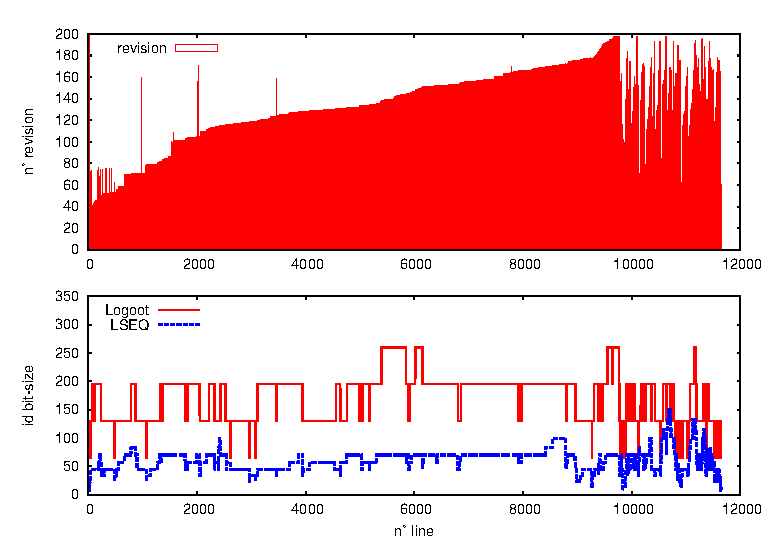
\includegraphics[width=\textwidth]{img/poste.eps}
  \caption{The Wikipedia page has 12k lines and is mostly edited at the
    end. The average bit-lengths of identifiers are $168.7$ and $61.24$ for
    \textbf{L} and \textbf{\NAME{}}$^\approx$ respectively.}
  \label{im:poste}
\end{subfigure}
\hfill
\begin{subfigure}[r]{0.47\textwidth}
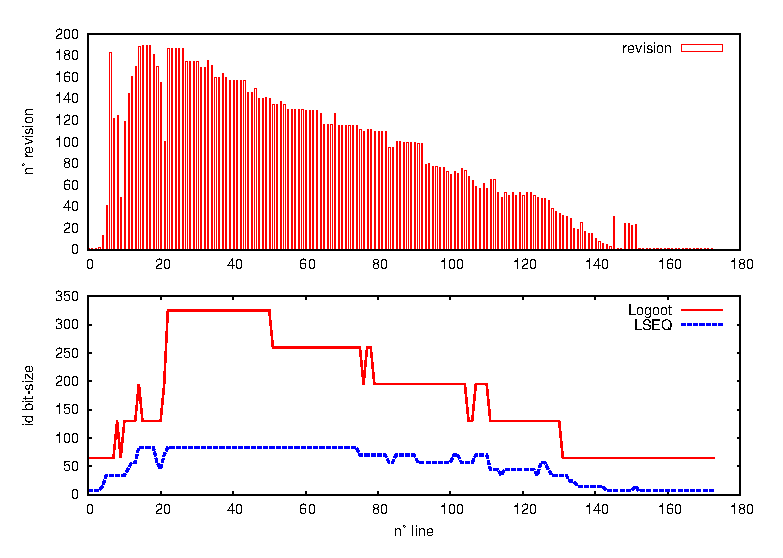
\includegraphics[width=\textwidth]{img/didyouknow.eps}
\caption{The Wikipedia page has 170 lines and is mostly edited at the
  beginning. The average bit-lengths of identifiers are $172.25$ and $51.99$
  $bit/id$ for  \textbf{L} and \textbf{\NAME{}$^\approx$} respectively.}
\label{im:didyouknow}
\end{subfigure}
\caption{The top spectrums reflect the editing behaviour performed on Wikipedia
  pages. The bottom figures shows the identifier bit-length assigned to each
  line. Two configurations: Logoot (\textbf{L}) and Round-Robin with base
  doubling (\textbf{\NAME{}}$^\approx$).}
\end{figure*}

\paragraph{Front Editing in Wikipedia}
\begin{asparadesc}
  
\item[Objective:] to highlight the importance of alternating the allocation
  strategies in \textbf{\NAME{}}$^\approx$. In other words, the
  \emph{boundary+} strategy of \textbf{L} is not sufficient to provide a safe
  allocation system. Finally, to show that \textbf{\NAME{}}$^\approx$
  outperforms \textbf{L} on documents edited at the beginning.

\item[Description:] we choose the Wikipedia
  page~\footnote{\url{http://en.wikipedia.org/wiki/Template_talk:Did_you_know}}. Since
  it is a ``talk'' page, it provides a discussion space. The users mostly
  inserted elements at the beginning of the document. Once again, we make the
  measurements on two configurations.
  \begin{inparaenum}[(1)]
    \item \textbf{L} with a single \emph{boundary+} strategy, and parameters
      set to $base=2^{64}$ and $boundary=1M$,
    \item \textbf{\NAME{}}$^\approx$ with the two allocation strategies
      \emph{boundary+} and \emph{boundary--}, and $base=2^{4+depth}$,
      $boundary=10$.
  \end{inparaenum}

\item[Result:] unsurprisingly, the figure~\ref{im:didyouknow} shows that using
  \textbf{L}, the identifiers bit-length increases very fast in the beginning
  of the document while it quickly stabilizes when \textbf{\NAME{}}$^\approx$
  is used. In Table~\ref{tab:didyouknow}, we observe that the average
  identifiers bit-length of \textbf{\NAME{}}$^\approx$ is $3.31$ times lower
  than the one of \textbf{L}.  The alternation of strategies allows
  \textbf{\NAME{}}$^\approx$ to quickly find a depth where allocation of
  identifiers will be efficient, and thereby to amortize previous depths where
  some spaces could have been wasted.  These observations confirm the results
  of section~\ref{ssec:components}.
  
  \item[Reasons:] \textbf{\NAME{}}$^\approx$ does not favour any editing
    behaviour thanks to its allocation strategies. On the opposite, \textbf{L}
    uses an allocation strategy designed to support end editing, thus, when
    the antagonist behaviour arises, the identifiers size grow very fast.
\end{asparadesc}

\begin{table}[h]
\addtolength{\belowcaptionskip}{-15pt}
  \begin{center}
    \begin{tabular}{|c|c|r|r|}
      \cline{3-4}
      \multicolumn{2}{c|}{} &\textbf{L} &\textbf{\NAME{}}$^\approx$\\
      \cline{3-4}
      \hline
      \multirow{2}{*}{id-length} & avg & $2.69$ & $5.29$ \\
      \cline{2-4}
     &  max & $5$ & $8$ \\
      \hline
      \hline
      \multirow{2}{*}{id-bit-length} & avg & $172.25$ & $51.99$\\
      \cline{2-4}
      & max & $320$ & $84$ \\
      \hline
    \end{tabular}
    \caption{Numerical values of experiments on the Wikipedia page edited at
      the beginning (corresponding to Figure~\ref{im:didyouknow}).}
    \label{tab:didyouknow}
  \end{center}
\end{table}

\subsection{Synthesis}

Experiments evaluated the contribution of each part of \NAME{} allocation
function. They demonstrated that each isolated component cannot achieve
sub-linear space complexity. However, their composition with random choice
among \emph{boundary+} and \emph{boundary--} and a base doubling can achieve
sub-linear space complexity in extreme setups. We also observe this gain on
real documents. Consequently, \NAME{} is suitable for building distributed
collaborative editors that deliver better performance and in a larger scope of
usage than state of art.


  \section{Related Work}
\label{sec:relatedwork}

Popular distributed collaborative editors such as Google
Docs~\cite{nichols1995high} rely on Operational Transformation approach
(OT)~\cite{sun1998operational,sun1998achieving}.  OT-based and CRDT-based
distributed editors follow the same global scheme of optimistic replication,
i.e., generate operations without locking, broadcast to others replicates and
re-execute. OT and CRDT mainly differ in their complexities:
\begin{inparaenum}[(i)]
\item OT-based editors have constant-time complexity at generation time and a
  complexity of $O(|H^{2}|)$ at re-execution time where $H$ is the log of
  operations. Performance of OT closely depend on the number of concurrent
  operations present in the system.
\item LSEQ sequence CRDT has a complexity of $O(k)$ for generation time and
  $O(k*log(n))$ for re-execution time where $n$ is the number of elements
  presents in the document and $k$ is proportional to size of
  identifiers. Unlike OT, the state of the document mainly determines the CRDT
  performance. \NAME{} significantly improves the performance of the sequence
  CRDTs by keeping $k$ small.
\end{inparaenum}

The tombstone class of sequence CRDT includes WOOT~\cite{oster2006data},
WOOTO~\cite{weiss2007wooki}, WOOTH~\cite{ahmed2011evaluating},
Treedoc~\cite{preguica2009commutative}, CT~\cite{grishchenko2010deep},
RGA~\cite{roh2011replicated}, \cite{Yu2012stringwise}. In these approach,
tombstones (or ``death certificates'') mark the deleted elements. They provide
a simple solution to solve problems of concurrent delete. A clear advantage is
to only require fixed-length identifiers, nonetheless the space complexity of
tombstone-based sequence CRDTs is linear compared to the number of insert
operations performed on the document.

Safely garbaging tombstones in a distributed system is costly because it
requires obtaining a consensus for this decision among all participants.
In~\cite{roh2011replicated, letia2009crdts}, they proposed some solutions
related to the garbage collecting mechanism in order to rebalance and/or purge
the model of the CRDT.  The purge~\cite{roh2011replicated} of tombstones
requires a full vector clock to keep track of updates on other replicas and to
be able to safely remove the tombstones. The \emph{core
  nebula}~\cite{letia2009crdts} approach intends to make the consensus
reachable, but constrains the topology of the network and uses an expensive
\emph{catch up} algorithm.

The variable-size identifiers class of CRDT includes
Logoot~\cite{weiss2009logoot} and Treedoc~\cite{preguica2009commutative}. These
CRDTs use growing identifiers to encode the total order among elements of the
sequence. In the worst case, the size of identifiers is linear in the total
number of insert operations done on the
document~\cite{ahmed2011evaluating}. Logoot and
Treedoc~\cite{preguica2009commutative} have different allocation
strategies. Treedoc has two allocation strategies:
\begin{inparaenum}[(i)]
\item the first strategy allocates an identifier by directly appending a bit on
  one of its neighbour identifier.
\item The second strategy increases the depth of this new identifier by $\lceil
  log_2(h)\rceil +1 $ (where $h$ is the highest depth of the identifiers
  already allocated) and allocates the lowest value possible with this growth,
  in prevision of future insertions.
\end{inparaenum}

Logoot's \emph{boundary} strategy and Treedoc's second strategy are very
similar, both in their goals and their weaknesses. They assume an editing
behaviour in the end, and therefore they become application dependent.
Compared to Logoot and Treedoc, \NAME{} is adaptive and significantly enlarges
the applicability of sequence CRDTs.

In~\cite{ahmed2011evaluating}, they compared most sequence CRDTs and one OT in
an experimental setup. RGA and Logoot obtained best overall performances. In
this paper, we completed experiments with more extreme cases and demonstrated
that \NAME{} outperforms Logoot.


  \section{Conclusion}

In this paper, we presented an original allocation strategy for sequence CRDTs
called \NAME{}. Compared to state of art, \NAME{} is adaptive, i.e., it handles
unpredictable different editing behaviour and achieves sub-linear space
complexity. Consequently \NAME{} does not require a costly protocol to garbage
or re-balance identifiers, and is suitable for building better distributed
collaborative editors based on sequence CRDTs.

Three components compose \NAME{}:
\begin{inparaenum}[(1)]
  \item a base doubling,
  \item two allocation strategies \emph{boundary+} and \emph{boundary--},
  \item a random strategy choice.
\end{inparaenum}

Although each component cannot achieve sub-linear complexity, the conjunction
of three components provides the expected behaviour. Experiments show that
even if \NAME{} makes a bad strategy choice for one level in the tree, this
choice will be overwhelmed by the gain obtained at next levels.

% Ifdoubled base, by making the
% assumption of a good allocating strategy employed, permits to obtain a
% sub-linear upper-bound for the size of identifiers generated. Also, the random
% alternance of strategies ($boundary+/boundary-$) ensures that a good strategy
% will eventually be employed. Individually, these components have huge
% weaknesses but their composition overcomes their respective defects.

The \NAME{} approach is generic enough to be included in other variable-size
sequence CRDTs. Current experiments were done with a Logoot basis because it
does not require tombstones and therefore is less dependent of the editing
behaviour. But we believe that Treedoc's heuristic could be improved with this
allocation strategy.

Future works include a formal demonstration of the empiric poly-logarithmic
upper-bound in space complexity which implies a probabilistic study of the
worst-case. The idea is to prove that its probability of happening is
negligible. We also plan to study if concurrency affects LSEQ results, i.e., if
each site makes different allocation choices concurrently, does it impact
\NAME{} performances? Finally, we aim to study if using documents spectrum
knowledge and machine-learning approaches can outperform random strategy
choice.


  
\section{Acknowledgements}
We would like to thank the anonymous reviewers for their comments and
suggestions which not only strenghten this work but also led to answer some
thorny issues about future work.



%% Bibliographie
  \bibliographystyle{abbrv}
  \raggedright
  \bibliography{bibliographie}
%  \addcontentsline{toc}{chapter}{Bibliographie} 
  \clearpage
  
\end{document}
